\clearpage
\section{Data Collection and Processing}

AssetWorx has the ambition to disrupt the industry of road maintenance. In order to do so, AssetWorx wants to collect the data themselves. This serves multiple benefits. First, they are the owner and can use the data however they want right now but also with future processing. Secondly, it makes them interdependent of suppliers. For instance, if the supplier developers their own models to classify defects, they can directly sell the information to the maintainer. 

Data collection is done by installing a sensor box in a car. This sensor box consists of an AutoPi (3rd generation) \cite{AutoPi} connected with a webcam. The following sources of data are available:
\begin{itemize}
\item CAN bus: the standard protocol for transmitting data within a car \cite{ISO11898}. Its one of the five protocols used in on-board diagnostics (OBD-2) in vehicle diagnostics. The OBD-2 connector is mandatory in all cars since 2004 \cite{EU1998}. This port allows the AutoPi to real-time log data about such as RPM, speed, engine temperature etc. It depends on the specific vehicle which data is available.
\item Global Positioning System (GPS) for location.
\item Real-time clock for accurate timing.
\item Accelerometer which measures accelerations of the car in x, y and z direction.
\item Camera which records road's surface.
\end{itemize}

For my thesis I'll be driving a car fitted with an AutoPI and collect data throughout writing my thesis. Currently AssetWorx lacks the infrastructure and architecture to process the collected data. In order to systematically process the collected data various data pipelines are designed. These pipelines can be holistically viewed as as a data platform architecture. Implementation of this platform is done on Google Cloud Platform (GCP) by using certain services GCP provides. 

To orchestrate these steps, Prefect is used \cite{Prefect}. Prefect is a dataflow automation tool. Although it is designed to orchestrate large workflows over various machines for large scale processing, it also comes with easy to use library to run workflows / pipelines locally.

\subsection{Layers of the Architecture}

The designed approach takes a modern data platform architecture with loosely coupled layers. 

\begin{figure}[H]
\begin{center}
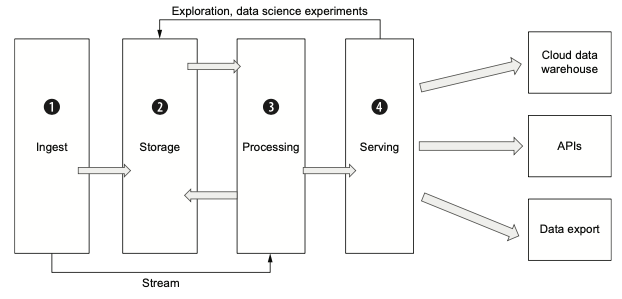
\includegraphics[width=\textwidth,keepaspectratio]{images/4_data/architecture-example.png}
\end{center}
\caption{Example layered architecture of data processing.}
\end{figure}

\begin{enumerate}
\item Data Ingestion: getting the data into the data platform. This is data collected by the AutoPI and the video recording. These sources are manually pulled and temporarily stored on my laptop before uploading the data. The data from the AutoPI can be directly uploaded. However, the video recording is first processed to anonymize PII data.
\item Data Storage: raw data within the platform is stored at Google Cloud Storage. Cloud storage doesn't impose any restrictions on types of file which can be uploaded and thus can store both the raw sensor data and visual data. Processing of data may produce a different form of data which can be stored at Cloud Storage or BigQuery.
\item Processing: data is processed to make it more useful. For instance, the Trips Pipeline distills distinctive trips from the data. Resulting trips are then stored back in the Storage layer.
\item Serving: data from the platform is served in a useful form which can be used to create models to make predictions. 
\end{enumerate}



In table \ref{tab:data-pipelines} all the data pipelines are listed with a description of their operation. In figure \ref{fig:data-pipelines} the pipelines are visualized. Most data pipelines are relatively straightforward and don't need further explanation than listed in the table. However, there are a few interesting data pipelines that are further described below.

% Please add the following required packages to your document preamble:
% \usepackage{booktabs}
% \usepackage{graphicx}
\begin{table}[h!]
\resizebox{\textwidth}{!}{%
\begin{tabular}{@{}p{0.25\linewidth}llp{0.6\linewidth}@{}}
\toprule
Name &
  Source &
  Destination &
  Description \\ \midrule \midrule
Ingest Accelerometer &
  \begin{tabular}[c]{@{}l@{}}Landing\\ Cloud Storage (jsonlines)\end{tabular} &
  \begin{tabular}[c]{@{}l@{}}Landing\\ BigQuery\\ \textit{raw\_accelerometer}\end{tabular} &
  Loads raw records from Cloud Storage into BigQuery table. \\ \midrule
Ingest GPS &
  \begin{tabular}[c]{@{}l@{}}Landing\\ Cloud Storage (jsonlines)\end{tabular} &
  \begin{tabular}[c]{@{}l@{}}Landing\\ BigQuery\\ \textit{raw\_gps}\end{tabular} &
  Loads raw records from Cloud Storage into BigQuery table. \\ \midrule
Ingest Wegdeel &
  \begin{tabular}[c]{@{}l@{}}External\\ Postgis\end{tabular} &
  \begin{tabular}[c]{@{}l@{}}Landing\\ BigQuery\\ \textit{raw\_wegdeel}\end{tabular} &
  Loads road sections (wegdeel) from Postgis database into BigQuery table. \\ \midrule
Ingest Frames Labels &
  \begin{tabular}[c]{@{}l@{}}Landing\\ Cloud Storage (txt)\end{tabular} &
  \begin{tabular}[c]{@{}l@{}}Landing\\ BigQuery\\ \textit{raw\_frames\_labels}\end{tabular} &
  Loads manually label annotations into BigQuery table. \\ \midrule
Ingest Label Lookup &
  \begin{tabular}[c]{@{}l@{}}Landing\\ Cloud Storage (txt)\end{tabular} &
  \begin{tabular}[c]{@{}l@{}}Landing\\ BigQuery\\ \textit{raw\_label\_lookup}\end{tabular} &
  Loads manually label definitions into BigQuery table. \\ \midrule \midrule
Determine Trips &
  \begin{tabular}[c]{@{}l@{}}Landing\\ BigQuery\\ \textit{raw\_gps}\end{tabular} &
  \begin{tabular}[c]{@{}l@{}}Staging\\ BigQuery\\ \textit{stg\_gps}, \textit{stg\_trips}\end{tabular} &
  Parses from GPS records distinct trips the car has travelled (further described below). \\ \midrule
Snap Trips to Roads &
  \begin{tabular}[c]{@{}l@{}}Staging\\ BigQuery\\ \textit{stg\_trips}\\ \\ External\\ Bing\end{tabular} &
  \begin{tabular}[c]{@{}l@{}}Staging\\ BigQuery\\ \textit{stg\_trips\_snapped}\end{tabular} &
  Snap the preprocessed GPS records to actual roads (further described below). \\ \midrule
Filter Road Sections &
  \begin{tabular}[c]{@{}l@{}}Landing\\ BigQuery\\ \textit{raw\_wegdeel}\end{tabular} &
  \begin{tabular}[c]{@{}l@{}}Staging\\ BigQuery\\ \textit{stg\_road\_section}\end{tabular} &
  Filter the road sections that are actually in use. \\ \midrule
Create Label Lookup &
  \begin{tabular}[c]{@{}l@{}}Landing\\ BigQuery\\ \textit{raw\_label\_lookup}\end{tabular} &
  \begin{tabular}[c]{@{}l@{}}Staging\\ BigQuery\\ \textit{stg\_label\_lookup}\end{tabular} &
  Converts ingested definitions to lookup table in order to join with annotated frames.\\ \midrule
Video to Frames &
  \begin{tabular}[c]{@{}l@{}}Landing\\ Cloud Storage (mov)\end{tabular} &
  \begin{tabular}[c]{@{}l@{}}Staging\\ Cloud Storage (jpg)\end{tabular} &
  Extracts separate frames from the recorded video (1 frame per second).\\ \midrule
Video to Frames Bootstrap &
  &
  &
  Spawns off separate jobs to process all video files in parallel.\\ \midrule \midrule
Link Trip Coordinates with Road Sections &
  \begin{tabular}[c]{@{}l@{}}Staging\\ BigQuery\\ \textit{stg\_trips\_snapped}\\ \\ Staging\\ BigQuery\\ \textit{stg\_road\_section}\end{tabular} &
  \begin{tabular}[c]{@{}l@{}}Production\\ BigQuery\\ \textit{mrt\_trips}\end{tabular} &
  Joins the snapped trips with the cleaned road sections from the BGT. \\ \midrule
Calculate Road Section Windows &
  \begin{tabular}[c]{@{}l@{}}Production\\ BigQuery\\ \textit{mrt\_trips}\end{tabular} &
  \begin{tabular}[c]{@{}l@{}}Production\\ BigQuery\\ \textit{mrt\_road\_section\_windows}\end{tabular} &
  Calculates timestamps (windows) when each road section was entered/exited per trip. \\ \midrule
Load Frames Labels &
  \begin{tabular}[c]{@{}l@{}}Landing\\ BigQuery\\ \textit{raw\_frames\_labels}\\ \\ Staging\\ BigQuery\\ \textit{stg\_label\_lookup}\end{tabular} &
  \begin{tabular}[c]{@{}l@{}}Production\\ BigQuery\\ \textit{mrt\_frames\_labels}\end{tabular} &
  Joins annotated frames with lookup table. \\ \midrule 
Load Frames Metadata &
  \begin{tabular}[c]{@{}l@{}}Production\\ Storage\end{tabular} &
  \begin{tabular}[c]{@{}l@{}}Production\\ BigQuery\\ \textit{mrt\_frames\_metadata}\end{tabular} &
  Creates a metadata table on the extracted frames (e.g. source video, timestamp and size). \\ \midrule 
Ingest Experiment Labels &
  \begin{tabular}[c]{@{}l@{}}External\end{tabular} &
  \begin{tabular}[c]{@{}l@{}}Production\\ BigQuery\\ \textit{mrt\_experiment\_labels}\end{tabular} &
  Ingests separate labels annotated by experiment runs into BigQuery. \\ \midrule 
Anonymize &
  \begin{tabular}[c]{@{}l@{}}Staging\\ Cloud Storage (jpg)\end{tabular} &
  \begin{tabular}[c]{@{}l@{}}Production\\ Cloud Storage (jpg)\end{tabular} &
  Automatically detect PII data and blur the detected objects.\\ \midrule
Anonymize Bootstrap &
  &
  &
  Spawns off separate jobs to process all source files in parallel.\\ \bottomrule
\end{tabular}%
}
\caption{Overview of all the different data pipelines.}
\label{tab:data-pipelines}
\end{table}

\begin{figure}[h!]
\begin{center}
\makebox[\textwidth][c]{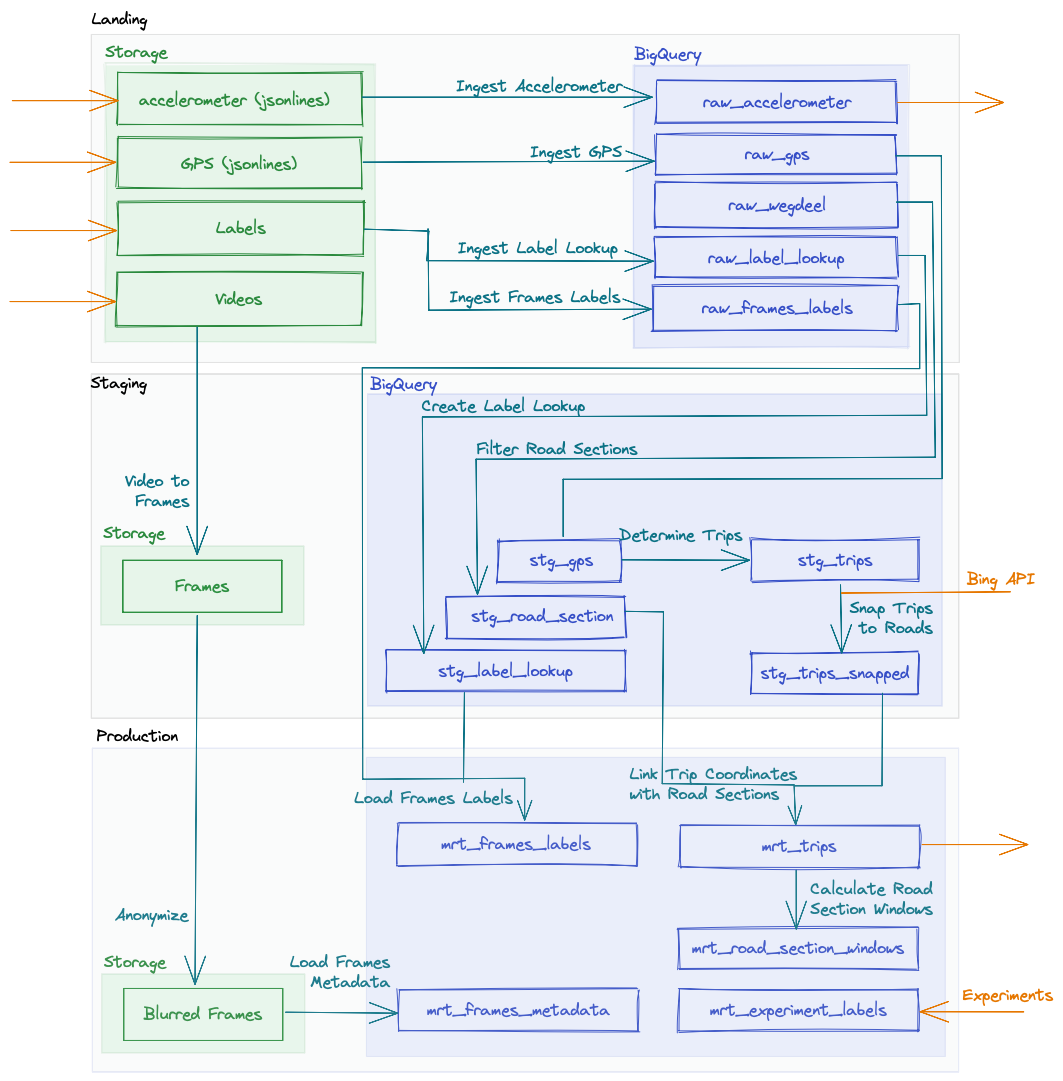
\includegraphics[width=1.2\textwidth,keepaspectratio]{images/4_data/data-pipelines.png}}
\end{center}
\caption{Visual overview of the various Data Pipelines.}
\label{fig:data-pipelines}
\end{figure}


\subsection{GPS Data}


\subsubsection{Determine Trips}
The GPS sensor records the location of the vehicle with 10 samples per second. After ingestion, this data is stored in raw form on Google Cloud Storage (GCS). The format is stored as json lines. A file format where aach line in the file is a single json document. Within this document the location of the vehicle is recorded with the respective time (see figure \ref{fig:gps-document} for an example). After the data is ingested in BigQuery, the GPS data is deduplicated and distinctive trips are detected with the following algorithm.

\begin{figure}[H]
\centering
\begin{minipage}{.35\textwidth}
  \centering
  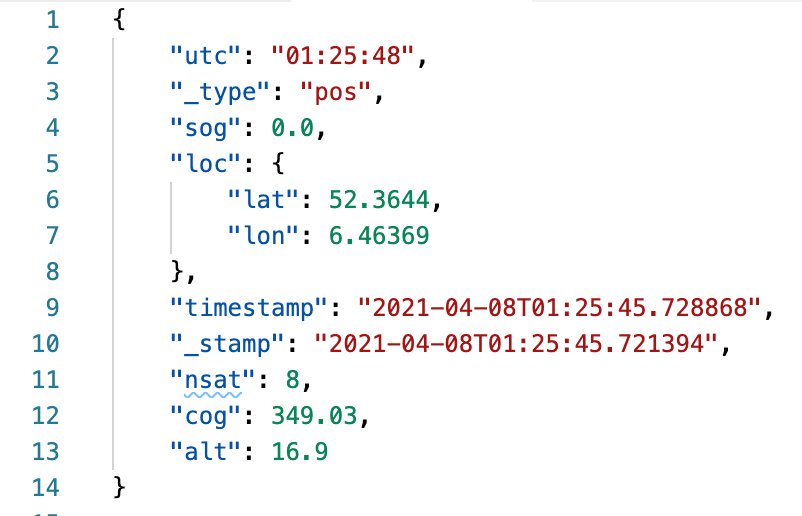
\includegraphics[width=\linewidth]{images/4_data/gps-example.png}
  \captionof{figure}{Single document describing GPS location. GPS data is recorded at 10 samples per second.}
  \label{fig:gps-document}
\end{minipage}%
\qquad
\begin{minipage}{.6\textwidth}
  \centering
  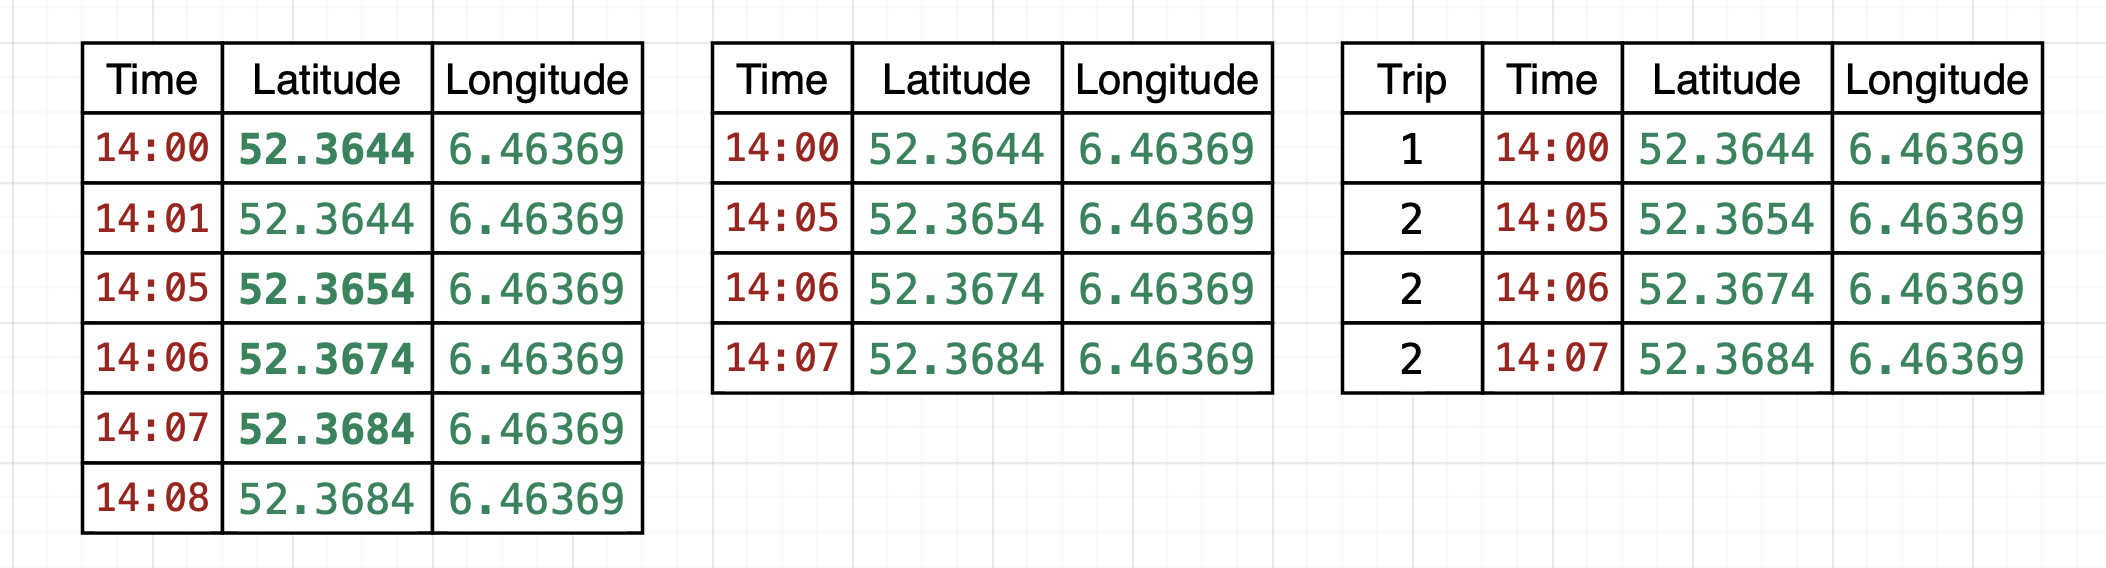
\includegraphics[width=\linewidth]{images/4_data/trip-detection.png}
  \captionof{figure}{Example of trip deduction algorithm. Left shows original data, center shows after deduplicating based on the location, right shows the resulting trips.}
  \label{fig:test2}
\end{minipage}
\end{figure}


\begin{enumerate}
\item Deduplication: the GPS sensor records location with 10Hz in raw form. If the car is stationary (e.g. traffic light), the data is still recorded, resulting in lot of duplicate records. The first step is to deduplicate the data. This is done by selecting the first record for each unique location in subsequent time series. 
\item Delta calculation: between each subsequent record the delta between time and distance is calculated. From these deltas, the speed is also calculated for metadata.
\item Detect trips: trips are detected from the consecutively records by finding records where the delta time is larger than 120 seconds (dwell time).
\item Reset trips: for each first record of a trip, the delta time, distance and speed are reset to zero. 
\item Cleanup trips: to cleanup invalid data, only trips are selected with more than 5 records of data and with at least 500 meters travelled in total.
\end{enumerate}


\subsubsection{Snap Trips to Roads}
The data collected by the GPS data might be noisy. As is known in literature, GPS data may drift over time meaning that GPS coordinates might not align with actual roads. For instance, some measurements may be positioned besides actual roads, see also figure \ref{fig:snap-trips}. This is an issue because we want to be able to overlay different trips over the same segment. This is done by anchoring on "road sections" which is further described below. However, it is impossible to anchor to a road section when subsequent GPS readings are beside the road section. In order to remedy this, the GPS coordinates are snapped to actual roads. The anchoring of the GPS coordinates is done with an external service. In this case that is "Snap Points to Roads" from Bing Maps (Microsoft) \cite{Snap-Points-to-Roads}, but any other external service can be used.
\begin{enumerate}
\item Given an unique trip (as previously determined).
\item Upload the coordinates to external service (Snap Points to Roads).
\item Link the snapped coordinates to the original coordinates.
\item Load the resulting trip in BigQuery.
\end{enumerate}

\begin{figure}[H]
\begin{center}
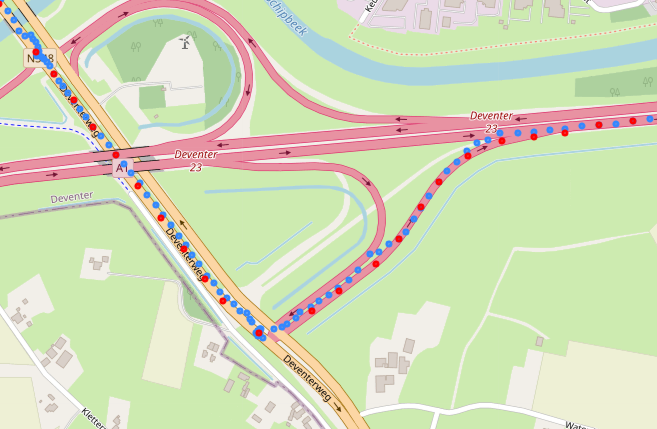
\includegraphics[width=.7\textwidth,keepaspectratio]{images/4_data/snap-trips.png}
\end{center}
\caption{Display of snapping coordinates to roads. The blue dots are the measured GPS coordinates, and the red dots are the inferred coordinates by external service. Note that some of the blue dots are on the wrong lane or beside any roads.}
\label{fig:snap-trips}
\end{figure}

\subsubsection{Link Trip Coordinates with Road Sections}
\textit{Basisregistratie Grootschalige Topografie} (BGT) is registry of large-scale object in the public space. This registry marks all locations and their area (in coordinates) of large-scale objects such as roads, buildings and territory. The BGT is regulated by law, and is mandatory for governments to use and maintain while operating with public space \cite{BGT}. Within the BGT roads are listed in "road sections". The size of a section varies to a single street bump in a town, to several hundred meters of highway. BGT is therefore a reliable source to anchor equal trips over the same roads.
\begin{enumerate}
\item Given an unique trip.
\item Join it with the road sections where the snapped coordinates are contained within a section.
\end{enumerate}


\subsubsection{Calculate Road Section Windows}
The sensor data (visual and accelerometer) can only be linked with location data through the recorded timestamps. In order to link the sensor data across different trips, the anchored road sections are used as described above. 
\begin{enumerate}
\item Given an unique trip.
\item Find the points when a road section was entered/exited by checking when the road section differs in subsequent records (similar to trip detection algorithm).
\item Get the first and last timestamp.
\end{enumerate}


\subsection{Visual Data}


\subsubsection{Video to Frames Pipeline}
The road's surface is recorded with an iPhone 12 mini. The video is recorded in 4K at 60 frames per second (FPS). The phone is located in a generic used phone holder attached to the windshield. \textit{TODO: image}. In order to further process the data, the frames are extracted from the recorded video. The algorithm can be seen as:
\begin{enumerate}
\item Given a path to location of video file
\item Download the video to temporary location
\item Decode the video file
\item Retrieve frames per second
\item For each second
\begin{enumerate}
\item Extract a single frame
\item Calculate the timestamp of this frame
\item Copy metadata from the video to to frame (also known as exif data)
\item Upload the frame to staging area
\end{enumerate}

\end{enumerate}
To speed up the pipeline, extraction of frames from the video and uploading the frame happen in separate threads. 


\subsubsection{Frame Extractor Bootstrap}
The video files are stored in a private cloud, accessible only by the author to safeguards any privacy concerns. The Video to Frames pipeline operates on a single video. However, during data collecting, data from many trips are collected. Therefor there are many video files to convert. This pipeline operates in a Kubernetes cluster to make the processing of video files concurrently. It works as follows:
\begin{enumerate}
\item List all video files 
\item For each video file
\begin{enumerate}
\item Asynchronously spawn of Video to Frames pipeline
\end{enumerate}
\end{enumerate}


\subsubsection{Anonymization Pipeline}
Although not intentional, the camera may record other cars, persons and other PII data. To safeguard any privacy concerns, the data is stored on a private cloud only accessible to the author. Before any further processing is done, the data is anonymized. This is done by blurring PII data from the individual frames. Detection of PII data happens with pre-trained YOLOv5 model \cite{Jocher2021}. This model is trained on COCO dataset, and thereby capable of detecting various classes among which are: [person, bicycle, car, motorcycle, airplane, bus, train, truck, boat]. The algorithm works as follows:
\begin{enumerate}
\item Given a path to staging area of extracted frames (for single video)
\item List the frames in that path
\item For each frame
\begin{enumerate}
\item Download the frame to temporary location
\item Run YOLOv5 to detect PII data
\item Blur the detected bounding boxes
\item Upload the anonymized frame to production area
\end{enumerate}
\end{enumerate}


\subsection{Accelerometer Data}


\subsubsection{Resampling}
The AutoPI was configured to sample the accelerometer data at 12.5Hz. However, the software only writes changes to the data i.e. duplicate consecutive records were not recorded. This means that the retrieved data has a variable sampling rate. This presents a problem to further processing operations. For instance, Fourier transformation is impossible on variable sampling rate. Therefore, the data is resampled at 12.5Hz by interpolating the recorded samples. This is done by fitting a B-spline curve for the given samples, and from that spline the data is uniformly sampled. 12.5Hz was set as sampling frequency as it was the configured setting for the AutoPI. 

This is shown in figure \ref{fig:accelerometer-resampling}. The top blue graph shows the raw readings from the accelerometer. The bottom graph shows the resulting data after resampling. Notice that the interval between readings of the top graph is variable, whereas the bottom is evenly spaced every 80 milliseconds (12.5Hz).

\begin{figure}[H]
\begin{center}
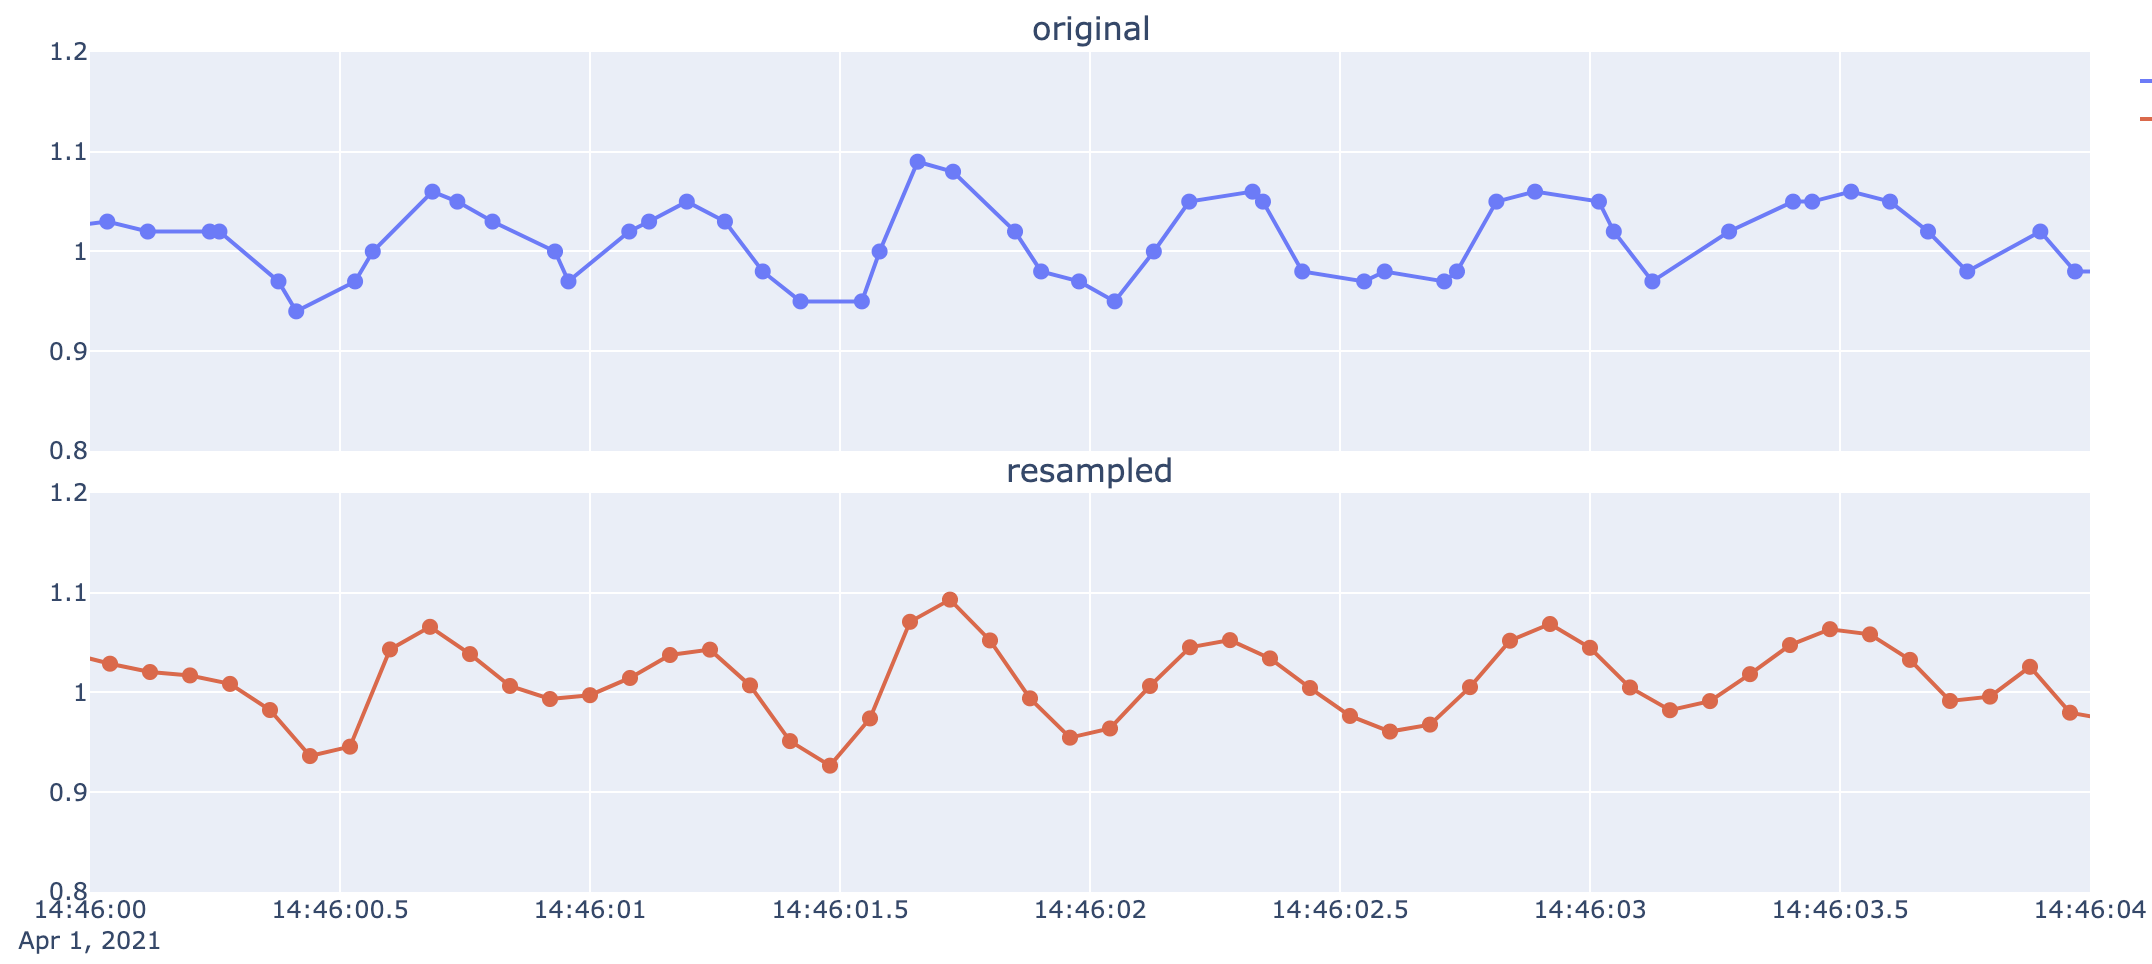
\includegraphics[width=\textwidth,keepaspectratio]{images/4_data/accelerometer-resampling.png}
\end{center}
\caption{Top graph displays the raw data from the accelerometer. Bottom graph displays the accelerometer data after resampling.}
\label{fig:accelerometer-resampling}
\end{figure}


\subsubsection{Realignment}
The AutoPI is installed in the vehicle, however the coordinate system of the accelerometer may not coincide with that of the vehicle. Meaning, when the vehicle drives over a bump it is expected to see a acceleration in vertical axes. However, it is likely that the readings are misaligned. Before the data can be useful, the coordinate system of the sensor must be aligned with that of the vehicle. To fix this issue, a method was developed to automatically align the coordinate systems. This makes it possible to generalize the collection of data to any vehicle. The process consists of two steps: first the coordinate system is aligned on the vertical axes, subsequently the horizontal plane is aligned. The idea is straightforward, the accelerometer sensor $a_s$, is measured when a known force is exerted on the vehicle, $a_v$. With this data it is possible to align the coordinate systems using Euler angles. This is also displayed below in figure \ref{fig:align-vectors}. For reference, in this thesis a Cartesian coordinate system is used. Where X, Y, Z refers respectively to the longitudinal, lateral and vertical axes.

For the first step, aligning the vertical Z-axes, the known force is the gravity of the earth. When the vehicle is stationary, the expected force is $a_v = (0, 0, g)$. Detecting when the car is stationary is done by checking the GPS data. Ideally, only accelerometer data is used when the vehicle is on a level surface. As we don't have access to this information, we rely on taking the average of many samples, as it can be assumed that on average the vehicle is mostly stationary on a flat surfaces. 

In order to align the coordinate systems, we can use Euler angles. The task is to calculate 3 dimensional rotation matrix $R_z$ to align vector $a_s$ onto vector $a_v$ in the vertical Z-axes. It is calculated as follows.

\begin{flalign*} 
\text{Let } v &= a_s \times a_v \\
\text{Let } c &= a_s \cdot a_v \\
\text{Let } skew &=
\begin{bmatrix} 0 & -v_3 & v_2 \\ v_3 & 0 & -v_1 \\ -v_2 & v_1 & 0 \end{bmatrix} \\
R_z &= I + skew + skew^2 \frac{1}{1 + c}
\end{flalign*}

The second step is to align the coordinates system in the longitudinal X-axes. Again, we take readings of the accelerometer when a certain force is expected. In this case when the car is braking, the expected acceleration is $a_v = (-x, 0, g)$, where $x$ depends on the deceleration of the vehicle. Braking windows are selected based on the derived speed from the GPS coordinates. As the vertical axes is already aligned, we need to calculate a two dimensional rotation matrix $R_x$ to align vector $a_s$ onto vector $a_v$ in the longitudinal X-axes. 

\begin{flalign*} 
\cos \theta &= a_s \cdot a_v \\
\sin \theta &= a_s \times a_v \\
R_x &= \begin{bmatrix} \cos \theta & -\sin \theta & 0 \\ \sin \ \theta & \cos \theta & 0 \\ 0 & 0 & 1 \end{bmatrix} \\
\end{flalign*}

Given the rotation matrix $R_z$ and $R_x$, the data from the accelerometer can be aligned for all subsequent readings. In the figure \ref{fig:align-vectors} the two-step method is visually presented.


\begin{figure}[H]
\begin{center}
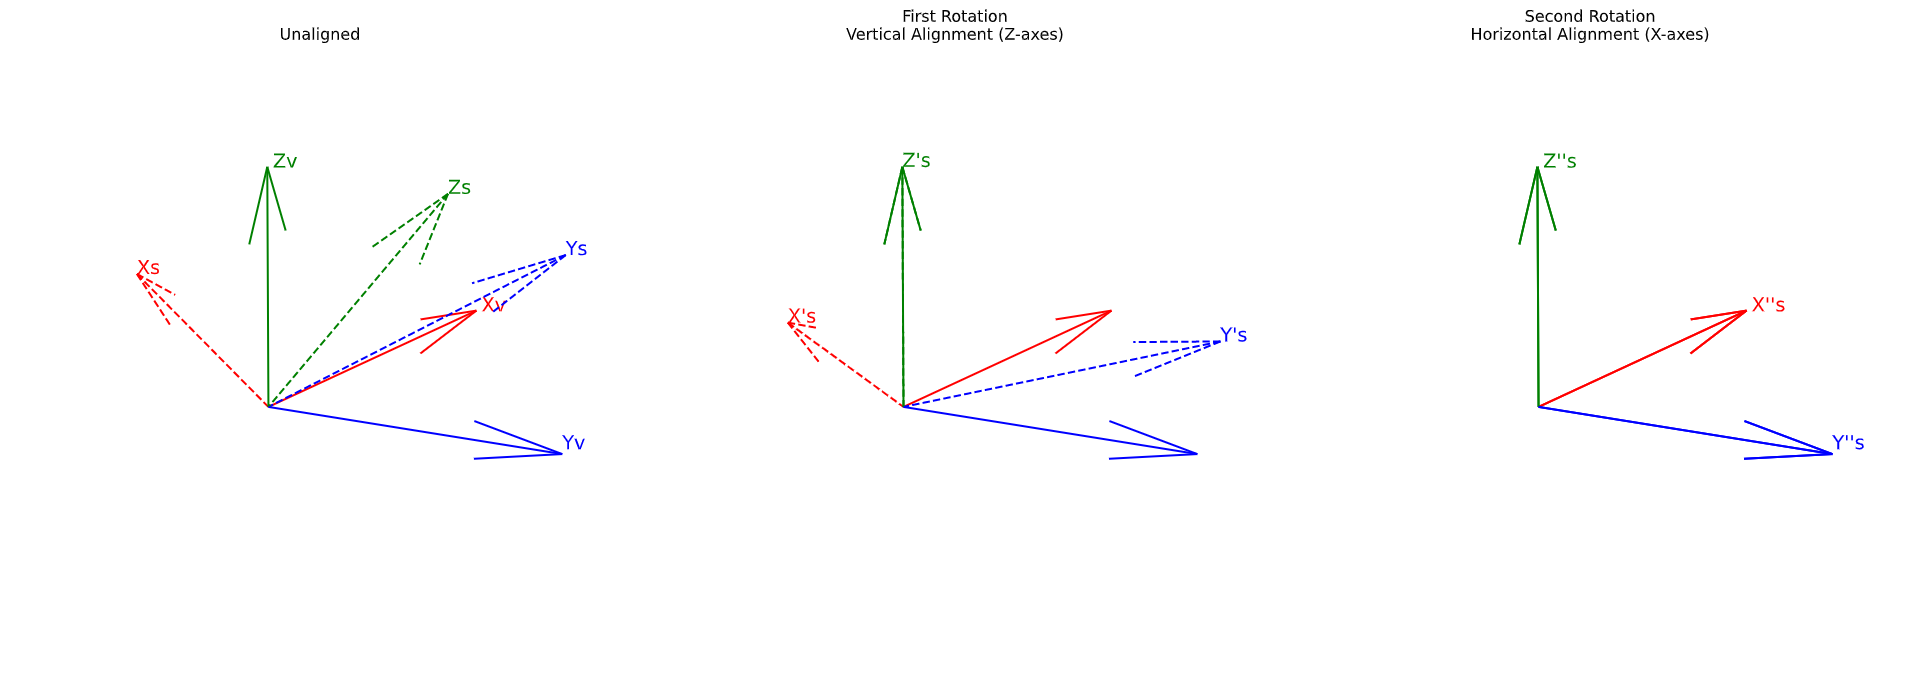
\includegraphics[width=\textwidth,keepaspectratio]{images/4_data/accelerometer-alignment.png}
\end{center}
\caption{Figure displaying the process of aligning the axes. Zv is the Z-axes for the vehicle, Zs is the Z-axes for the sensor. Left: shows the original, unaligned situation. Middle: shows the situation after aligning the Z-axes. Right: shows situation after aligning the X-axes.}
\label{fig:align-vectors}
\end{figure}


 
